\documentclass{beamer}
%\usepackage{beamerthemeBerkeley}
% Use either the one above or the one below
\usetheme{CambridgeUS}
%\usepackage{graphicx,color}
%\usepackage{lmodern}
%\usepackage{colortbl}

\usepackage{tikz}
%\usetikzlibrary{matrix,arrows,positioning}
\usepackage{algpseudocode}

\title{Datalog extensions}
\author{Simone de Oliveira Santos}
%\date{\today}

\begin{document}

\frame{\titlepage}

%\section[Outline]{}
%\frame{\tableofcontents}

\section[Distributed SociaLite]{Distributed SociaLite: A Datalog-based language for large-scale graph analysis}

\subsection{Introduction}

\frame{
	\frametitle{Distributed SociaLite: A Datalog-based language for large-scale graph analysis}

	\textbf{Motivations}
	
	\begin{itemize}
		\item With the rise of world-wide social networks, many graph-oriented databases are now available.
		\item The large graphs need large-scale distributed systems to be processed.
		\item MapRedure and Pregel are examples of techniques that masks the complexity of distributed processing.
		\item Pregel adopts a vertex-centric programming model, this feature makes it one of the most well-known languages designed in response for social network analysis.
	\end{itemize}
	
}

\frame{
	\frametitle{Distributed SociaLite}

	\begin{itemize}
		\item SociaLite makes it possible for an implementation that hides the low-level complexity in distributed execution from the programmers.
		\item It is built upon the sequential SociaLite as a new language extension and optimization for large-sale graph analysis on distributed machines.
	\end{itemize}
}

\frame{
	\frametitle{Contributions}
	
	\begin{description}
		\item [Data distributed through sharded tables] The programmer does not have to worry about distributing the computation and managing the communication. Instead, he simply specifies how data are to be decomposed across the machines.
		\item [Parallel recursive aggregate function] Delta stepping is effective for parallelizing the shortest path algorithm. Now it is made available to any recursive monotone aggregate functions.
		\item [Efficient approximation] SociaLite automatically returns partial answers as it process the Datalog rules using semi-naive evaluation. Delta stepping and Bloom filters are used to deliver partial results.
	\end{description}
}


\frame{
	\frametitle{Single-source paths problem}
	
	\begin{figure}
		\centering
		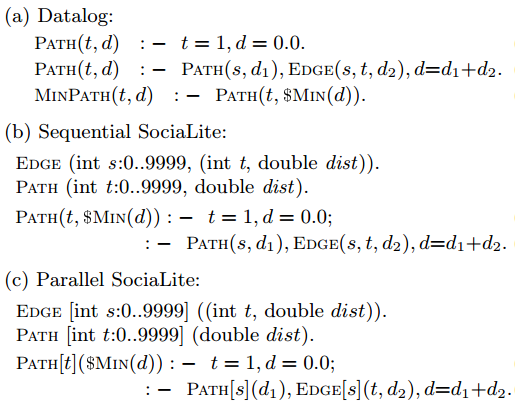
\includegraphics[width=8cm]{comparison.png}
	\end{figure}
	
}

\frame{
	\frametitle{Parallel SociaLite extensions}

	\begin{itemize}
		\item Ask programmers to indicate how the date are to be partitioned across the distributes machines.
		\item It introduces a \textit{location operator}([]) to be applied to the first column of a data declaration.
		\item The declaration PATH[int $t$](double $dist$) specifies that PATH is a relation with two columns and that the table is horizontally partitioned, or \textit{sharded}.
	\end{itemize}
	
}

\subsection{Data distribution in SociaLite}
\frame{
	\frametitle{Data distribution in SociaLite}
	
	\begin{itemize}
		\item \textbf{Shards}, each containing a number of rows, are placed on different machines in a distributes system.
		\item The value of the first column in a relation is the \textit{shard key}, and it dictates where the relation is located. 
		\item The function \textsc{ShardLoc}($r,x$) returns the machine number based on the value of the \textit{shard key} $x$ in relation $r$.
	\end{itemize}

}

\frame
{
	\frametitle{Range-based and hash-based shards}

	\begin{itemize}
		\item There are two kinds of sharding: \textbf{range-based} and \textbf{hash-based}
		\item If the first column of a sharded array has a range, then the range is divided up into consecutive subranges and evenly distributes across the machines.
	\end{itemize}
	
	Supose the shard key $x$ in relation $r$ has hange $l..u$, then	
	
	\begin{equation*}
		\textsc{ShardLoc}(r,x) =\left\lfloor\frac{x-l}{\left\lceil\frac{u-l+1}{n}\right\rceil}\right\rfloor
	\end{equation*}
	
	Where $n$ is the number of machines in this system.
}

\frame
{
	\frametitle{Range-based and hash-based shards}

	\begin{itemize}
		\item If no range is given, it is used a standard hash function to map the shard key to a machine location.
		\item The range of the hashed values is also evenly distributed across all the machines.
		\item The location operator is also used in rule specifications to make it apparent to the programmer where the operands and results are placed.
	\end{itemize}
	

}

\subsection{Distribution of computation}
\frame{
	\frametitle{Distribution of computation}

	\begin{center}
		\textsc{Bar}[int $x:0..9999$](int $z$). \\
		\textsc{Baz}[int $z:0..9999$](int $y$). \\
		\textsc{Foo}[int $x:0..9999$](int $y$). \\
		\textsc{Foo}[$x$]($y$) :- 	\textsc{Bar}[$x$](z),	\textsc{Baz}[$z$]($y$) \\
	\end{center}

	The rule specifies that data \textsc{Bar}[x](z) are to be transfered to a machine with ID \textsc{ShardLoc}(\textsc{Baz},$z$), where join operation with \textsc{Baz}[$z$]($y$) is performed. \\
	
	The result from the join operation is then transferred back to a machine with ID \textsc{ShardLoc}(\textsc{Foo},$x$).
}

\subsection{Batching the messages}
\frame
{
	\frametitle{Batching the messages}

	The compiler rewrites the rules so that all the computation is performed on local data, and communication is necessary only for sending the result to the right machine. \\
	

	\begin{block}{}
		\textsc{Bar}'[int l:0..9999](int x, int z). \\

		\textsc{Bar}'[$z$]($x,z$) :- \textsc{Bar}[$x$]($z$). \hspace{6.5cm} (1)\\

		\textsc{Foo}[$x$]($z$) :- \textsc{Bar}'[$z$]($x,z$), \textsc{Baz}[$z$]($y$) \\

	\end{block}

	The rule (1) distributes all the relations of \textsc{Bar} on each machine into a sharded relation \textsc{Bar}'. Each shard destined for a different machine, \textsc{ShardLoc}(\textsc{Bar}',$z$) $\neq$ \textsc{ShardLoc}(\textsc{Bar},$x$), is sent to the appropriate machine in one message.
	
}

\subsection{Parallel Execution Engine}
\frame{
	\frametitle{Distributed system architecture}
	
	The SociaLite parallel machine consists of a master machine which interprets the Datalog rules and issues work to a collection of slave machines.
	
	\begin{block}{Fault-tolerant distributed file system}
	If one or more workers fail, the intermediate states are restored from the latest check point and the evaluation is resumed from that point.
	\end{block}
	
}

\frame{
	\frametitle{Distributed system architecture}
	
	\begin{figure}
		\centering
		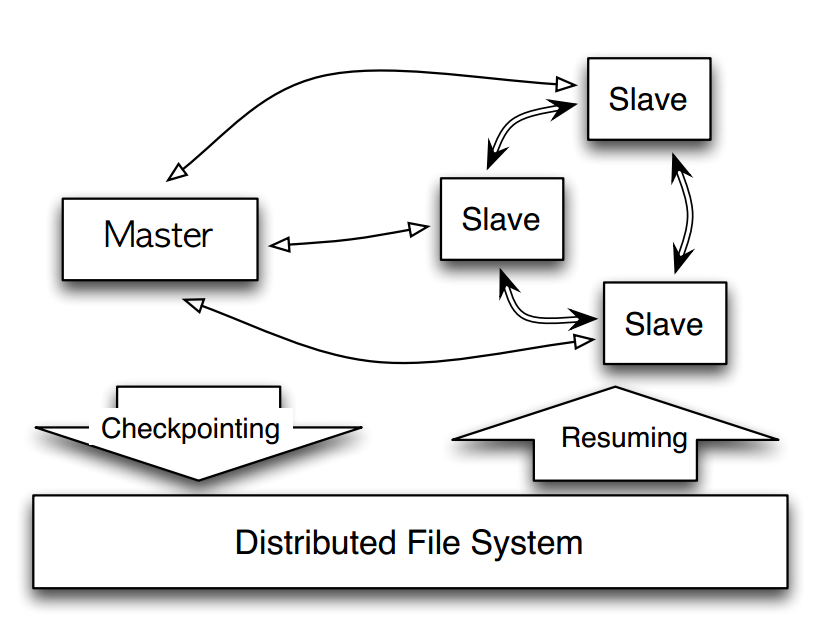
\includegraphics[width=7cm]{Distr_system_architecture.png}
	\end{figure}

}

\frame{
	\frametitle{Distributed system architecture}
	
	\begin{itemize}
		\item The master compiles the SociaLite program into a dependence graph, where each node corresponds to a join operation and each edge represents a data dependence.
		\item After finding the strongly connected components, the master organize all the nodes within a stratum into epochs.
		\item Recursive strongly connected components are each placed into their own epoch.
		\item Non-recursive rules can be combined into epochs with the constraint that dependences across the epochs form an acyclic graph.
	\end{itemize}
	
}

\frame{
	\frametitle{Distributed system architecture}

	\begin{itemize}
		\item The master then visits the epoch graph in a topological order and instructs the slaves to work on an epoch at a time.
		\item Each slave node repeatedly executes the rules upon the arrival of communication from other nodes and updates the internal tables or sends messages to remote nodes as needed.
		\item Protocol used to detect when the slaves complete an epoch:
		\begin{itemize}
			\item slaves report its idle status to the master if there are no rules to execute and no more data to send.
			\item Upon receiving an idle status from all the slaves, the master confirms with each slave that it is still idle with the same last reported timestamp. This process is repeated until confirmation from each slave are received. 
		\end{itemize}
	\end{itemize}
}

\frame{
	\frametitle{Multiple cores}

	\begin{itemize}
		\item Each sharded table is further \textit{subsharded}, with each subsharded $32n$ ways, where $n$ is the number of cores supportes on the machine.
		\item SociaLite breaks up tasks into units that operate in a subshard at a time and are placed in a dynamic task queue.
		\item Each machine has a manager responsible for:
		\begin{itemize}
			\item accepting epoch assignment
			\item report and confirming idle status with the master
			\item accepting inputs
			\item placing the corresponding tasks on the work queue
			\item sending data intended fir other machines
		\end{itemize}
		\item Each worker fetches tasks from the work queue, performs the task and updates the resulting data tables.
	\end{itemize}
	

}

\frame
{
	\frametitle{Multiple cores}
	
	\textbf{Two optimizations to minimize the synchronization overhead}
	\begin{itemize}
		\item Non-recursive epochs are further broken down into \textit{sub-epochs} whose rules are totally independent of each other. Synchronization is necessary only to enforce mutual exclusion between result update operations.
	\end{itemize}
	
	\begin{figure}
		\centering
		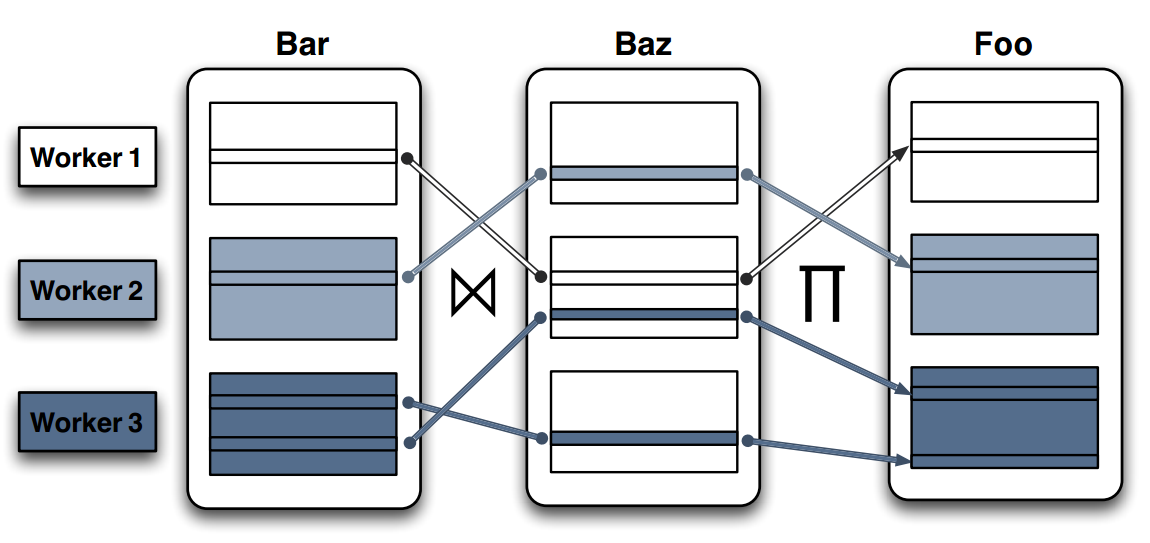
\includegraphics[width=10cm]{parallel_evaluation.png}
	\end{figure}
}

\frame
{
	\frametitle{Multiple cores}
	
	\textbf{Two optimizations to minimize the synchronization overhead}
	\begin{itemize}
		\item No synchronization is necessary if the updated shard is guaranteed to be accessed by only one worker.
	\end{itemize}
	
	\begin{figure}
		\centering
		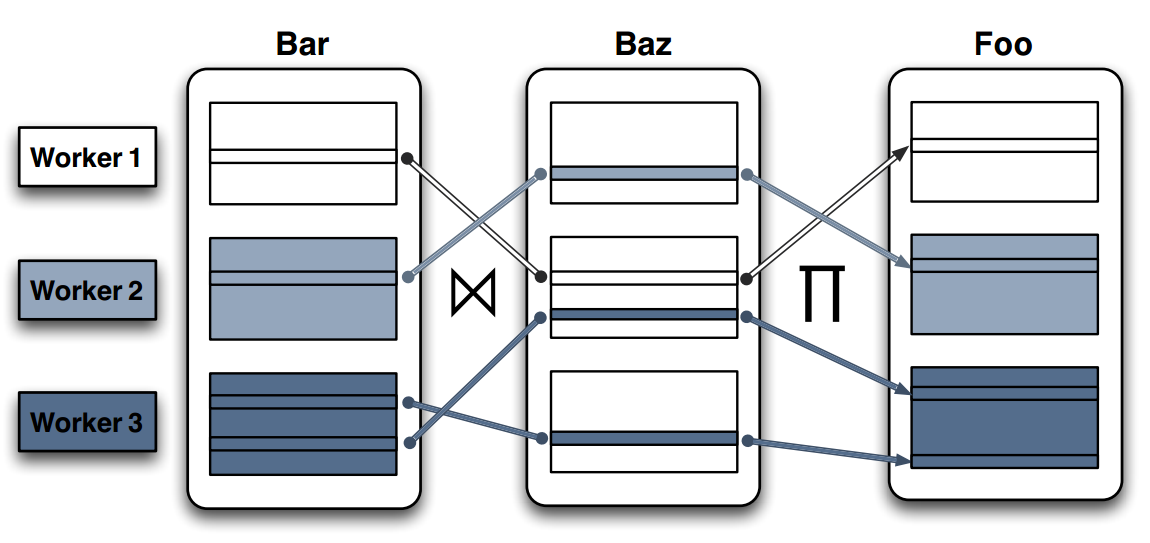
\includegraphics[width=9cm]{parallel_evaluation.png}
		\caption{Rule \textsc{Foo}[$x$]($y$) :- \textsc{Bar}[$x$]($z$), \textsc{Baz}[$z$]($y)$.  }
	\end{figure}
}

\subsection{Parallelizing recursive aggregate functions}
\frame
{
	\frametitle{Parallelizing recursive aggregate functions}
	
	\begin{itemize}
		\item The sequential SociaLite compiler uses a priority queue to keep track of all the newly tuples to be evaluated.
		\item By operating on the lowest values the solution converges quickly to the greatest fix point, yielding a behavior similar to that of Dijkstra's shortest-paths algorithm.
		\item \textbf{It is not suitable for distributed SociaLite to use priority queue, as it will serialize the evaluation of aggregate functions.}
	\end{itemize}
	
}

\frame
{
	\frametitle{Parallelizing recursive aggregate functions}
	
	\begin{itemize}
		\item \textbf{Delta Stepping} has shown to be effective in computing shortest paths for large-scale graphs.
		\item The parallel implementation of Delta Stepping algorithm gives near linear speedup (shown in a experimental study).
		\item Distributes SociaLite have generalized this technique and incorporate it into the compiler.
	\end{itemize}

}


\subsection{Approximation Computation}
\frame{
	\frametitle{Approximation Computation}

	\begin{itemize}
		\item Results of a query in a large-scale graph may also be very large.
		\item For the sake of a faster response, it might be desirable to provide partial results to the user instead of waiting until all results are available.
		\item The semi-naive evaluation of SociaLite rules supports approximate computation trivially.
		\item Approximation is achieve by simply terminating each epochs of the execution before the fix point is reached.
	\end{itemize}

}


\frame{
	\frametitle{Bloom-Filter based approximation}
	
	\begin{block}{The Bloom filter}
		Used as a means to provide a quick approximation to the case where the final result may be relatively small, but the intermediate results are large.
	\end{block}
	
	\begin{itemize}
		\item When intermediate sets gets too large to be represented exactly, Bloom filter is used to represent them compactly. 
	\end{itemize}
	
	\begin{block}{Friend of a friend program}
		\textsc{Foaf}($n,f_{2}$) :- \textsc{Friend}($n,f$), \textsc{Friend}($f,f_{2}$). \\
		\textsc{FoafSum}(n,\$\textsc{Sum}(a)) :- \textsc{Foaf}($n,f_{2}$), Attr($f_{2},a$)
	\end{block}

}

\end{document}
